% !TEX program = xelatex

\documentclass[10pt,draft]{article}
\usepackage{amsmath}
\usepackage{titlesec}
\usepackage{graphicx}
% \usepackage{sidecap} % captions on the side
\usepackage{floatrow}
\usepackage[scientific-notation=true]{siunitx} % siunits and numbers
\usepackage{caption}

\usepackage{helvet}
\renewcommand{\familydefault}{\sfdefault}
\usepackage{subcaption}
\usepackage[color=cyan!40,obeyFinal]{todonotes}
\usepackage[margin=0.5in]{geometry}
\usepackage{cleveref}
\usepackage{microtype} %sexy kerning
\usepackage{color} % colors
\usepackage{ulem} % strikethrough
\usepackage{ifdraft}
\usepackage[	backend=biber,
		style=numeric-comp,
		sorting=none]{biblatex}
\addbibresource{ace.bib}
\floatsetup{heightadjust=object}

\date{}
\titleformat{\subsection}
  {\normalfont\fontsize{11}{17}\sffamily\bfseries\slshape}
  {\thesubsection}
  {1em}
  {}
\DeclareSIUnit\Molar{\textsc{m}}
\setcounter{secnumdepth}{4} % paragraph acts as subsubsubsection

\newcommand{\subsubsubsection}[1]{\paragraph*{#1}}

% only show strikethrough text when draft (broken, comment out for draft)
% \renewcommand{\xout}[1]{\ifdraft{\xout{#1}\fi}{}}
% toggle for displaying instructions
\newif\ifinstr
\instrtrue

%If true, display \instr wrapped text, but only if draft mode on
\newcommand{\instr}[1]{\ifdraft{\ifinstr {\color{cyan}\emph{#1}} \fi}{}}

%pKa formatting
\newcommand{\pKa}{p$K_\mathrm{a}$\ }
\newcommand{\pH}{p$\mathrm{H}$\ }

\begin{document}
\listoftodos[Indexed list of activities pertaining to labor that will be performed in the short-term future]\newpage
\section*{\centering Specific Aims}
Among the most fundamental molecular interactions in biology are those of small molecules with their macromolecular partners.
\textbf{Endogenous small molecules play the role of messengers in many signaling pathways of the cell, and small molecule drugs interact with proteins in signaling cascades to modulate their function.}
Understanding their interactions is vital to understanding many biological systems, and critical to drug development efforts.
Despite having catalogued many of the physical driving forces behind small molecule recognition, \textbf{there are enormous gaps in our knowledge preventing us from articulating a quantitative, predictive understanding of small molecule affinities and selectivities for biomolecules.}

In principle, \textbf{alchemical free energy calculations} provide a framework for quantitatively describing all aspects of the thermodynamics of small molecule recognition. However, deficiencies in our quantitative understanding of binding create large challenges in the ability of these calculations to reproduce experimental affinities in many systems, holding back their use in probing function and aiding design.
In this proposal, we address \textbf{three of the most significant open challenges in the quantitative modeling of small molecule recognition}.

\subsection*{Aim 1. Establish a correct quantitative treatment of alchemical free energy calculations for binding of charged ligands}
The predominant soluble form of many drugs and endogenous small molecules is charged.
Yet, retrospective studies and predictive challenges show current free energy methods fail for charged species\cite{Rocklin2013b,Muddana2014a}.
A number of corrections for calculations with charged ligand species have been proposed\cite{Reif2013a,Rocklin2013a, Lin2014a}, but (1) consensus, and (2) a good model system to test and to confirm theory are lacking.
We propose using a computationally and experimentally tractable model system---the association of small-molecule guests with high-affinity supramolecular hosts---as a way to test, validate, and refine both theory and algorithms applicable to charged ligands.
The experimental datasets collected here will allow us to \textbf{ perform free energy calculations}, and to \textbf{ evaluate proposed corrections} in order to refine theory and algorithms as necessary.
We will utilize \textbf{ isothermal titration calorimetry (ITC) experiments}, which provide a “gold standard” biophysical assay for binding affinities.
We will additionally develop Bayesian approaches to accurately \textbf{ quantify measurement uncertainty} and allow for model-error propagation. \textbf{Without quantified uncertainty, it is not possible to distinguish between experimental errors and errors in theory}.

\subsection*{Aim 2. Quantify the magnitude of protonation state effects on binding}
\textbf{Proteins and many small-molecule drugs contain titratable moieties that can change protonation state upon binding} or sample mixtures of protonation states, often in a conformation-dependent manner.
While detailed biophysical studies of a few specific model systems have demonstrated that these effects can contribute several kcal/mol in binding affinity, \textbf{the true scope and magnitude of the problem in ligand recognition in general is completely unknown}.

We will use computational techniques to conduct a survey to assess the importance of protonation state issues in protein-small molecule interactions across a range of systems of pharmacological interest.
Existing \textbf{ \pKa prediction tools will be benchmarked against experimental small molecule \pKa data}, and then \textbf{ used for constant-\pH alchemical free energy calculations}.
We will perform complementary experiments on a tractable but disease-relevant system---kinase catalytic domains that can be expressed in \textit{E. coli}---using \textbf{ ITC experiments in buffers of different ionization enthalpies that allow for deconvolution of binding and protonation states effects}.

\subsection*{Aim 3. Develop a framework for alchemical free energy calculations to describe weak association and cooperative ligand binding}
Weak binding and association of multiple ligands are ubiquitous interactions in biological and pharmaceutically relevant systems.
In addition, drug discovery approaches such as fragment-based ligand design depend predominantly on a reliable method for integrating data from biophysical experiments with modeling for these situations.
We will \textbf{ extend the framework of alchemical free energy calculations}  to include the potential for \textbf{ multiple (possibly weak) binding events } using a \textbf{ semi-grand canonical ensemble formalism}.

As a model system, we will use the pharmacologically relevant protein \textbf{ human serum albumin } (HSA), known to bind many small molecules (sometimes multiple species at a time) to a variety of distinct binding sites.
We will  \textbf{ overcome deficiencies in theory } by both developing new Bayesian ITC experimental analysis techniques to select among theoretical association models, as well as simulating ITC data directly from semi-grand canonical ensemble simulations.

\subsection*{} % Add some spacing

Completion of the work will provide modeling strategies for non-trivial challenges in protein-ligand association that currently have no working solution, as well as illustrate the scope of challenges that remain.

\section*{Research Strategy - Significance}
\instr{General background, significance in terms of basic science and disease relevance.}

\todo[inline,color=magenta!40]{section on charged ligands}

\subsection*{Shedding light on the unknown contributions of protonation state changes to protein-ligand binding affinity}
To model protein-ligand association, using the correct protonation state can be key to success \cite{Polgar2005a,Wittayanarakul2008a}. But what if there is not a single protonation state that contributes to the binding affinity?

With the exception of a few known cases\cite{Aleksandrov2007a,Czodrowski2007a,Steuber2007a,Czodrowski2007b}, the ubiquitousness of protonation state changes and the magnitude of their contribution to binding affinities is completely unknown. Large contributions to ligand binding affinity are potentially neglected by the standard approach which neglects mixtures of protonation states of the ligand and protein during alchemical free energy calculations.

Take for instance the case of kinase inhibitor imatinib (marketed as Gleevec), for which is hinted that protonation state changes may play a role in determining its selectivity for Abl protein kinase\cite{Lin2013a}. These effects have to be quantified if one's goal is not just to answer what determines the selectivity of imatinib, but also to accurately calculate its binding affinity using alchemical free energy calculations.

\subsection*{Human serum albumin: a binder of many small molecules ligands}

Human serum albumin (HSA) is a protein with multiple binding sites that bind a wide variety of ligands \cite{He1992a,Kragh-Hansen2002a,Sulkowska2002a}. Its binding sites are asymmetric\cite{He1992a, Curry1998a} and one expects there to be difference in binding affinity of a ligand for each site\cite{Sudlow1976a}.

\todo[inline,color=lime!40]{refer to HSA figure with binding sites}

Because of the many small molecule interactions of HSA, it is expected to be of great importance to the bioavailability of small molecules \cite{Metcalfe2010a}. It is known to bind several drugs\cite{SJOeHOLM1979a,Bannwarth1996a,Sulkowska2002a,Ghuman2005a,Perez2007a}, as well as dietary supplements\cite{Pal2013a}. It is also essential for the bioavailability of endogenous small molecules such as hormones \cite{Pardridge1986a}, and toxins such as cardiac glycosides\cite{Smith1985a}. 

\subsection*{Association of multiple weak binders is relevant to fragment based drug discovery}
Multiple association is also relevant to fragment based drug discovery. The discovery of fragments that bind weakly to proteins and then combining them has been a useful method for experimental high-throughput screens. \cite{Hajduk2007a}. The association of these fragments is hard to model computationally, because of the challenges associated with modeling weak interactions. For instance, because of the absence of a strong signal that two compounds are ``bound'' to each other, it can be hard to define binding\cite{Gilson1997a}. 

Using a semi-grand ensemble formulation, tighter binding is automatically achieved by combining multiple fragments, since it is governed by the chemical potential of the bound state. The more favorable the binding, the stronger the potential will drive towards binding more fragments. This as opposed to simulations of single fragments and attempting to measure binding affinity, or extensive (and expensive) simulations of many fragment combinations, without a priori knowledge of good combinations. 

\todo[inline]{How common are charged ligands? How does it affect calculations when we don't correct them?}
\todo[inline]{Need to optimize fragment combinations in situ. Reduce screening costs?}
\todo[inline]{Amount of ligands that undergo protonation state changes}

\section*{Research Strategy - Innovation}
\instr{Explain how your proposal differs from what others have tried.}
\subsection*{Reliable uncertainty estimates of isothermal titration calorimetry results by using Bayesian statistics}
The ABRF-MIRG'2 study revealed the disturbing fact that the uncertainty of ITC experiments is underestimated by several orders of magnitude by conventional analysis methods\cite{Myszka2003a}. Panel D of \Cref{figure:abrf-mirg2} indicates a statistical uncertainty of at least 10\% in the estimation of extinction coefficients between all participants of the study, which correlates linearly with errors in the concentrations of the solutions prepared by each lab. This error is propagated into the estimates of binding stoichiometry, affinity and enthalpy  (Panels A, B and C of \Cref{figure:abrf-mirg2}).

By only performing technical replicates  and no repeat experiments, the true uncertainty can not be quantified, hence no hypothesis can be supported from any single experiment\cite{Vaux2012a}. That said, one can get an estimate of the uncertainty by performing Bayesian inference on experiments. For this reason, we propose the useage of Bayesian statistics as a means of uncertainty estimation as opposed to errors from model fit based on single or replicate experiments. Bayesian ITC\texttrademark can contribute to get more value out of single experiments by allowing for uncertainty quantification in concentrations of solutions. 

\thisfloatsetup{capposition=beside,
capbesideposition={center,right}}
\begin{figure}[H]
	\centering
	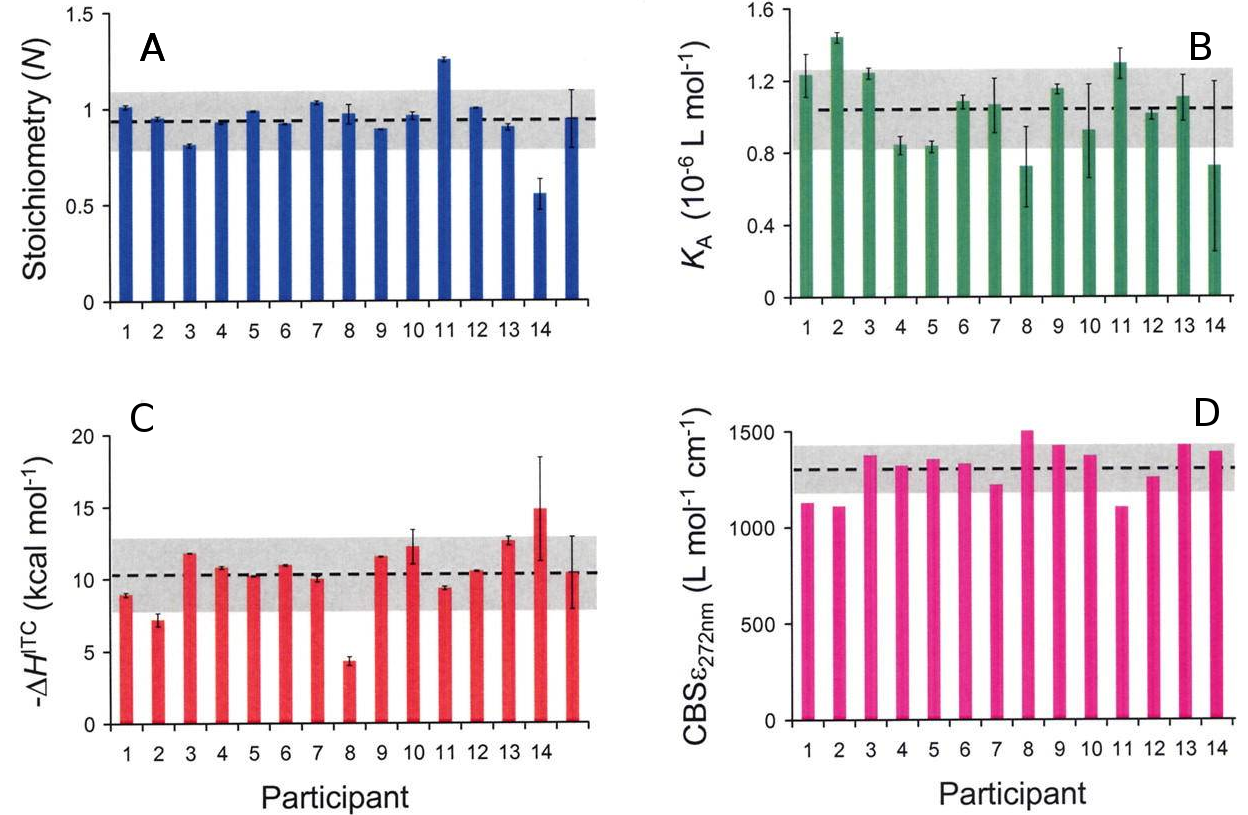
\includegraphics[width=0.49\textwidth]{figures/cbs_ca_II.PNG}
	\caption{Binding measurements from the ABRF-MIRG'2 study that considered binding of CBS to carbonic anhydrase using \textbf{ITC as performed by 14 labs shows individual error estimates that are orders of magnitude under the actual error.} A: Predicted stoichiometry of binding. B: Association constant $K_\mathrm{A}$. C: enthalpic contribution to binding. D: Measured extinction coefficient of ligand CBS, as reported by the 14 participants.\cite{Myszka2003a}}
	\label{figure:abrf-mirg2}
	\todo[inline,color=green!40]{need more detail here on what this data shows. can describe that same sample was distributed to 14 laboratories to measure affinity by ITC and that reported errors were orders of magnitude smaller than actual experimental variation. Also helpful to boldface first sentence of caption that succinctly summarizes figure. like ``Current ITC data analysis approaches drastically underestimate true experimental error.''}
\end{figure}

\subsection*{Quantifying and assessing correctness of poorly studied charge contributions to alchemical free energy calculations}
That there is a problem describing charged ligands in alchemical free energy calculations has been pointed out multiple times in the past\cite{Rocklin2013b,Muddana2014a}. 
For this reason, several possible ways of correcting this have been suggested \cite{Reif2013a,Rocklin2013a}. A quantitative comparison is lacking, and the correctness of these methods has not been established. 
By providing an experimental dataset with small and quantified uncertainty, we can provide a comparison of these methods that gives reasonable certainty to whether observed errors are experimental in origin, or are an error in the alchemical free energy theory. 
We can then not only provide a qualitative comparison on whether the models can possibly reproduce experiments, but will have a quantitative estimate of whether they produce the correct result.

These corrections may also prove to be necessary when performing constant-\pH calculations, where protons carrying single units of charge may come into and leave the simulation system as dictated by their chemical potential. Having a proven way of dealing with these protonation events will enable hypothesis driven research backed up by reliable simulation results.


\subsection*{Provide new frameworks for semi-grand canonical ensemble free energy calculations}
Currently, there is no available framework to perform alchemical free energy calculations that can sample binding free energy in the semi-grand canonical ensemble, allowing for multiple ligands to associate. We propose to extend the available toolset of the computational chemist with semi-grand canonical ensemble methods that enable the calculation of binding affinities of multiple ligands to multiple sites. As opposed to simulating a single ligand at multiple sites, this way we can correctly take into account cooperativity in binding when multiple ligands associate with a single protein.

Furthermore, frameworks that deal with constant-\pH methodology compatible with alchemical free energy calculations are 


\section*{Research Strategy - Approach}
\instr{Approach: More specific background information. Describe in detail the experimental design and research methods to be used. Technical hurdles to be overcome should be mentioned. Alternative approaches should be given for experiments that may not be feasible. Discussion of expected or possible results and their interpretation. Best format for each specific aim: a) rationale, b) methods, c) expected results, d) alternatives. Theory aims should follow a similar structure where possible.}

\todo[inline]{Explain Bayesian statistics (what detail?)}
\todo[inline]{Define some generic Bayesian models for ITC}


\subsection*{Aim 1. Establish a correct quantitative treatment of alchemical free energy calculations for binding of charged ligands}
\subsubsection*{Rationale}
The soluble form of many drugs and endogenous small molecules is charged. Yet, retrospective studies and predictive challenges show current free energy methodology fails for charged species\cite{Rocklin2013b,Muddana2014a}.
A number of corrections for calculations with charged ligand species have been proposed, but (1) consensus, and (2) a good model system to test and to confirm theory are lacking\cite{Reif2013a,Rocklin2013a, Lin2014a}. We will perform experiments using a Bayesian methodology to obtain a robust dataset. We will then \textbf{ perform alchemical free energy calculations to compare proposed corrections}.

\textcite{Reif2013a} use a thermodynamic cycle to define a raw charging contribution to binding free energy,
\begin{align}
	\Delta\Delta A^\mathrm{raw}_\mathrm{chr} = \Delta\Delta A^\mathrm{raw}_\mathrm{chr}(\mathrm{bound}) - \Delta\Delta A^\mathrm{raw}_\mathrm{chr}(\mathrm{free}) \quad,
\end{align}
which according to the authors must be corrected for four independent terms, shortly summarized:
\begin{itemize}
  \item $\Delta A_\mathrm{pol}$, for using a finite system, arising due to periodic boundary conditions and truncated potentials, or solvent models with inaccurate dielectric permittivity.
  \item $\Delta A_\mathrm{Psum}$, for inappropriate summation over individual point charges (``P-summation'') instead of over charges within individual solvent molecules  (``M-summation''), as well a constant offset when using Lattice-Sum methods. \cite{Kastenholz2006a}
  \item $\Delta A_\mathrm{dir}$, from using approximations such as reaction field or lattice-sum methods instead of full Coulombic electrostatic interactions.
  \item $\Delta A_\mathrm{exc}$, from neglecting interactions between (potentially incorrectly) excluded atoms 
\end{itemize}

\textcite{Rocklin2013a} uses similar corrections.

\emph{the paper is 27 pages long and I haven't read it yet. Expecting similarities with \textcite{Reif2013a} because of the authors involved}
\todo[inline,color=magenta!40]{check out the rocklin paper with corrections}

Then, there is the approach of \cite{Lin2014a}. 


%\subsubsection*{Methods}
\subsubsubsection{Subaim 1.1: Develop a Bayesian analysis framework for isothermal titration calorimetry to allow for uncertainty estimation}
In order to test theoretical approaches such as free energy calculations, a robust experimental dataset is necessary to distinguish between fundamental issues with the model or experimental errors. 
We will develop Bayesian approaches to \textbf{accurately quantify measurement uncertainty and allow for model-error propagation}. 
\todo[inline]{Explain how to describe an ITC experiment in a Bayesian way, focussing on things like concentration uncertainty}
The simplest model of an ITC experiment of a ligand $\mathrm{X}$ binding to a macromolecule $\mathrm{M}$ consist of a series of $n$ injections, resulting in injection heats $q_n$,
\begin{align}
	q_n = V_\mathrm{cell} \Delta H \left( [\mathrm{MX}]_n - [\mathrm{MX}]_{n-1} \right) + \Delta H_0 \label{equation:liberated-heat}
\end{align}
where $V_\mathrm{cell}$ is the volume of the sample cell, $\Delta H$ is the standard molar enthalpy of binding, $[\mathrm{MX}]_n$ is the complex concentration in the sample cell after $n$ injections, and $\Delta H_0$ is an offset that captures effects such as dilution and mechanical heats of stirring.


Errors in the concentration of prepared solutions are a major source of uncertainty in ITC data. Not taking these into account can lead to orders of magnitude underestimation of the uncertainty of the experiments \cite{Myszka2003a,Tellinghuisen2011a}.

One way to take this into account is by doing repeat experiments in which all solutions are prepared anew for each replicate, instead of technical replicates \cite{Vaux2012a}. This however is time and material consuming, and therefore not a popular option among most scientists. 

To provide an accurate assessment of \textbf{error from single experiments}, we can \textbf{perform inference by applying a Bayesian approach}. The concentration uncertainty can be modeled using a prior probability distribution around the expected concentration. Using \textbf{Markov Chain Monte Carlo (MCMC)} \cite{Metropolis1953a,Hastings1970a}, we can then sample from a posterior probability distribution to estimate the actual concentration using\textbf{ Bayes' rule}

\begin{align}
	\mathcal{P}\left(\theta | \mathcal{D} \right) \propto \mathcal{P}\left(\theta\right) \mathcal{P}(\mathcal{D} | \theta)
\end{align}


% \begin{align}
% \mathcal{P} \left(\Delta G_\mathrm{bind}, \Delta H_\mathrm{bind}, \Delta H_0, [\mathrm{X_{syr}}], [\mathrm{M_{cell}}], \sigma \biggl{|} \prod\limits_{m=1}^{M}\{q_m\}^{N}\right) \quad,
% \end{align}
, where $\theta$ an independent set of thermodynamical parameters, and $\mathcal{D}$ are the experimental observations, such as the injection heats $q_n$. 

An example model could describe $\theta$ as
\begin{align}
 	\theta   =  \left\{ \Delta G_\mathrm{bind}, \Delta H_\mathrm{bind}, \Delta H_0, [\mathrm{X_{syr}}], [\mathrm{M_{cell}}], \sigma \right\}
\end{align}

where $\Delta G_\mathrm{bind}$ is the binding affinity, $\Delta H_\mathrm{bind}$ is the binding enthalpy, $\Delta H_0$ is the mechanical heat of injection and dilution, $[\mathrm{X_{syr}}]$ is the true syringe concentration, $[\mathrm{M_{cell}}]$ is the true cell concentration, and $\sigma$ is the measurement noise.

\todo[inline,color=gray!20]{explain how we prevent overfitting by using Bayesian methods}


The methodology will allow incorporation of multiple experiments, such as calibrations, to accurately separate out heat effects due to e.g. dilution of the chemicals used or mechanical effects of the injections.

% \begin{align}
% 	 \mathcal{P}\left(\Delta G_\mathrm{bind}, \Delta H_\mathrm{bind}, \Delta H_\mathrm{dil},\Delta H_\mathrm{mech}, [\mathrm{X_{syr}}], [\mathrm{M_{cell}}], \sigma \biggl{|} \prod\limits_{m=1}^{M}\{q_m\}^{N}\right) \quad,
% \end{align}

% for $N$ injections per $M$ experiments. Calibration experiments can provide more certainty by separating out parts of the effects, such as dilution.
\todo[inline]{Explain that we can incorporate multiple experiments}

\todo[inline,color=red!40]{Why do we need Bayesian ITC? what do we not get out of the current method? How to validate and test this. Mention MCMC}

\xout{Furthermore, we will construct baseline models using gaussian process regression with scikit-learn\cite{Pedregosa2011a}.}
\todo[inline,color=red!40]{skip experimental design?}

\xout{We can apply high dynamic range type experiments to perform trial experiments that allow us to find the order of magnitude of the affinity.
This estimate can then be used for experimental design, determining the optimum conditions for our experimental setup.
We will simulate the outcome of ITC experiments using MCMC and then perform them to validate the results.}

\todo[inline, color=black!40]{insert preliminary data figure as illustration of the type of data that we will be generating?}

\subsubsubsection{Subaim 1.2 : Obtain isothermal titration calorimetry data with quantified uncertainty for host-guest systems}

We will utilize ITC experiments, which provide a “gold standard” biophysical assay for binding affinities.
We propose using the association of small-molecule guests with high-affinity supramolecular hosts as a way to test, validate, and refine both theory and algorithms applicable to charged ligands.
We will use cucurbit[7]uril \cite{Lagona2005a} as a host, which is known to bind a series of cations within a range of affinities spanning several orders of magnitude \cite{Cao2013a} (see also \Cref{figure:host-guest}).

\todo[inline,color=blue!40]{What is the dynamic range of the affinities? Useful because it is in a similar range as those achievable by protein:small mol complexes. }
\todo[inline,color=red!40]{It is a good model system because it is easy to sample with MD, and very soluble for ITC.}

\thisfloatsetup{floatwidth=\textwidth,%
capposition=beside,%
capbesideposition=left,%
capbesidesep=none}
\renewcommand\subfloatrowsep{\hskip 0\columnsep} % figure separation is done here
\begin{figure}
  \centering
  \ffigbox[\textwidth]{
    \begin{subfloatrow}[3]%\useFCwidth
      \fcapside[\FBwidth]{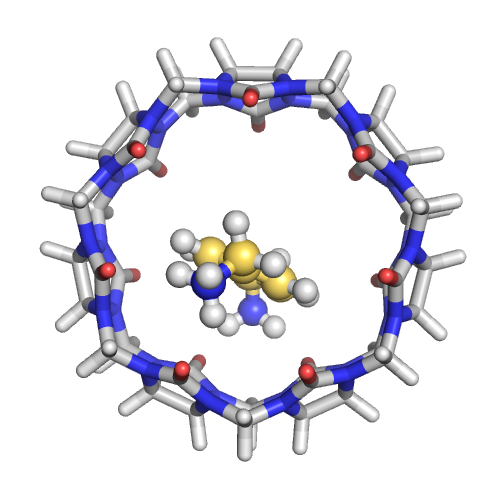
\includegraphics[width=.28\textwidth]{figures/guest11_top.png}}{\caption{}}%
      \subfloatrowsep
      \fcapside[\FBwidth]{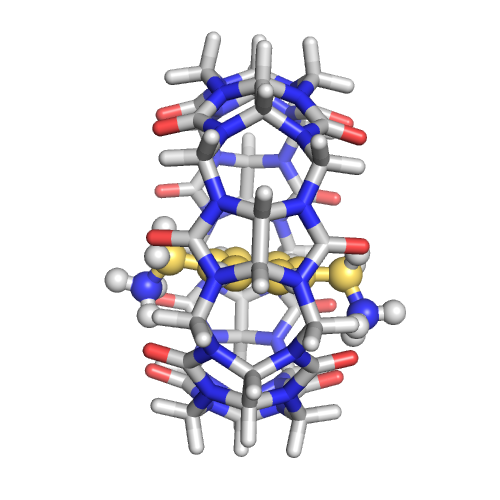
\includegraphics[width=.28\textwidth]{figures/guest11_side.png}}{\caption{}}%
      \subfloatrowsep
      \fcapside[\FBwidth]{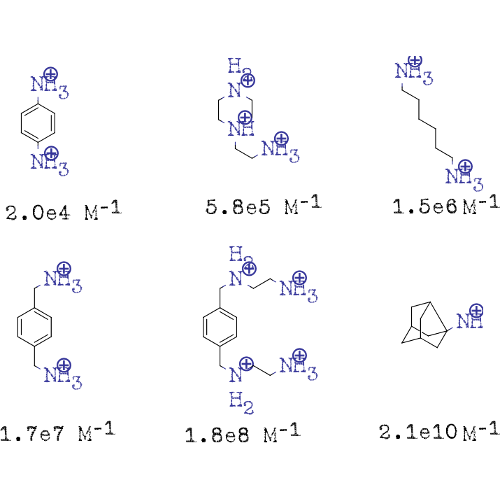
\includegraphics[width=.28\textwidth]{figures/guests_2d.png}}{\caption{}}%
    \end{subfloatrow}}
{\caption{\textbf{Cucurbit[7]uril (CB7) bound to several cationic guests from \textcite{Cao2013a}}. Different guests bind to the central cavity of CB7, though their affinity is determined by their geometry and size. (a) Guest 11 shown from the front, (b) from the side, (c) various guests and their $K_a$ values \cite{Cao2013a}. Figure prepared using Glide docking\cite{Halgren2004a,Friesner2004a,Friesner2006a,Schroedinger2014a} into crystal structure pdb:QQ7\cite{Feng2004a}.}\label{figure:host-guest}}
 
\end{figure}


\todo[inline, color=red!40]{Move this part to the general rationale, using host-guest as a given for all subaims}

\subsubsubsection{Subaim 1.3: Perform a quantitative comparison of suggested correction models to experiments to establish a correct treatment of charged ligands in alchemical free energy calculations}
We will compare several methods that correct for changes in net charge of the system in alchemical free energy calculations\cite{Reif2013a,Rocklin2013a}.
\todo[inline,color=cyan!40]{more detail needed. What are the essential ideas and why are they needed? Why is there disagreement? Might be another method from Benoit Roux.}

\todo[inline,color=green!40]{Explain the theory behind the two methods short, equations, show how they are different}
\missingfigure[figcolor=cyan!40, figwidth=0.8\textwidth]{Some illustation of alchemically removing salt pairs would be nice}

We will also test an additional model in which a neutral ligand:counterion pair is alchemically eliminated.

\subsubsection*{Expected results}
Estimates of the experimental uncertainty will allow us to distinguish model errors from variance in the experimental data.
The work will enable the comparison of the proposed charge correction models. 
The key question will then be whether any of the corrections  match up to experiment.
We will then be able to recommend a methodology to use when calculating the free energy of binding for charged species, enabling reliable simulations that are impossible to perform otherwise.
\subsubsection*{Pitfalls and alternatives}
\todo[inline,color=red!40]{What to do if the experimental uncertainty remains too high?}
\todo[inline,color=red!40]{What if none of the models agree with experiment?}
\todo[inline,color=red!40]{How do we pick a model if they all seem to agree? Can they all be correct?}
\todo[inline,color=red!40]{modulate strength of interactions by modulating salt concentration}

It is possible that all methods produce comparable results, in which case we will do... 
Issues with the molecular dynamics force field can influence the outcome of free energy methods in unpredictable ways. If the force field proves to be a troublesome factor, we will attempt to reparametrize our molecules to improve agreement with experiments.
\todo[inline,color=red!40]{ITC of neutral guest to point out force field problems.}

\subsection*{Aim 2. Quantify the magnitude of protonation state effects on binding}
\subsubsection*{Rationale}

Proteins and many small-molecule drugs contain titratable moieties that can change protonation state upon binding or sample mixtures of protonation states, often in a conformation-dependent manner.
\missingfigure[figcolor=orange!40, figwidth=0.8\textwidth]{imatinib protonation states}
While detailed biophysical studies of a few specific model systems have demonstrated that these effects can contribute several kcal/mol in binding affinity\cite{Aleksandrov2007a,Czodrowski2007a,Neeb2014a}, the true scope of the problem in ligand recognition in general is completely unknown.
\todo[inline,color=cyan!40]{explain Czodrowski example}
\textbf{The usual approach in modeling ignores these problems and assumes a single protonation state} for an entire system. Our aim is to \textbf{rectify this by using constant-\pH simulations} in the context of alchemical free energy calculations. Using computational \pKa prediction techniques to provide input for this framework will enable future consideration of these effects.
\todo[inline,color=red!40]{(You need to be clearer about the scientific goals here.  Perhaps be explicit in stating that you will create this tool and then assess how widespread these effects are in some problem class?  Also, might be clear that the pKa prediction techniques are for small molecules, and we need to evaluate which techniques will actually lead to useful intrinsic pKas of solvated ligands before their accuracy for use in simulating complexes can be assessed.)}
\xout{We will use computational techniques to conduct a large scale survey to broadly assess the importance of protonation state issues in protein-small molecule interactions across a range of systems of pharmacological interest.}
\todo[inline,color=yellow!40]{develop techniques to deal with the protonation state issues}
\xout{Existing \pKa prediction tools will be benchmarked against small molecule \pKa data, and then used together with Monte Carlo titration codes (both extant and developed for this project) to provide an estimate of the scope of the problem.}
\todo[inline,color=purple!40]{short explanation constant-\pH simulations}
\todo[inline,color=red!40]{explain kinase inhibitors}
% \subsubsection*{Methods}
\subsubsubsection{Subaim 2.1: Obtain reliable small molecule \pKa predictions for kinase inhibitors}
\todo[inline,color=red!40]{Couldn't we obtain reliable pKas by experimental measurement?  I think you just have to phrase this Aim title a bit more specifically so that someone reading this [and not reading your mind] can tell that you are trying to determine which small molecule pKa prediction methods [if any] could be useful to feed into a constant pH simulation framework for subsequent parts of this Aim.)}
Our aim is to \textbf{quantify the contribution of protonation state changes to binding} interactions. Experimental \pKa data is not widely available, so in part we will need to rely on computational \pKa prediction tools. We will \textbf{benchmark existing \pKa prediction tools}  using \pKa data obtained for a series of \textbf{kinase inhibitors} using a Sirius T3 instrument.
 \todo[inline,color=red!40]{(Note that this is a gold standard for giving macroscopic pKas using a combination of electrochemical and UV-metric titrations.)}

This will provide a means to select a tool that can adequately predict \pKa values for kinase inhibitors with similar chemical components.

Preliminary results suggest that \textbf{several kinase inhibitors have access to multiple states  at physiological \pH}. For instance, the intracellular \pH of most tumors is around 7.2 \cite{Griffiths1991a,Stubbs2000a}. Preliminary data in \Cref{figure:pka-kinase} indicates that a number of FDA approved kinase inhibitors have \pKa values close to the physiological \pH.
\begin{figure}[H]
	\centering
	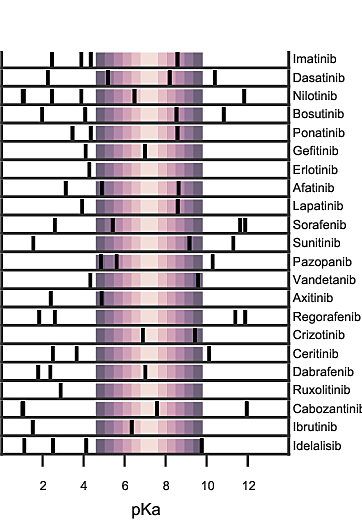
\includegraphics[width=0.27\textwidth]{figures/inhibitor-pKas.png}
	\caption{Protonation states accessible to FDA approved kinase inhibitors. Colors indicate accesibility of states at \pH 7.2 within blocks of $k_BT$ units of energy, where darker means more units of $k_BT$ away from the accesible region. Preliminary data obtained using Epik.\cite{Shelley2007a,Greenwood2010a}}
	\label{figure:pka-kinase}
	\todo[inline,color=green!40]{show some ligands, highlight sites, or even protein}
\end{figure}

Among the small molecule \pKa prediction tools considered will be \textbf{MoKa}\cite{Milletti2007a}, \textbf{Jaguar}\cite{Bochevarov2013a}, and \textbf{Epik}\cite{Shelley2007a,Greenwood2010a}.
MoKa generates \pKa{}s based on atomistic descriptors, defined by the surrounding atoms. The descriptors are based on molecular interaction fields calculated using GRID \cite{Goodford1985a} for a library of 3D fragments, but can succesfully be applied on 2D structures.
Schrodinger's Jaguar provides means of estimating \pKa values using quantum mechanical methods.
Epik uses Hammett Taft linear free energy approaches\cite{Perrin1981a} for predicting \pKa values .

\subsubsubsection{Subaim 2.2: Idenification of kinase-inhibitor combinations with potential protonation state effects}
To accurately incorporate \pKa effects into our simulations, we also need to consider that the \pKa of protein residues may change on binding of a ligand. 
\todo[inline,color=red!40]{what will you actually do in this subaim, what will the result be?}
Using kinases as model systems, we will survery small molecule-kinase interactions using MCCE\cite{Song2009a}, which will be extended to incorporate small molecules in its calculations.
We will make a selection of crystal structures from the protein data bank (PDB)\cite{Berman2000a} of kinases with inhibitors bound. 
We can then selecting for systems that show potential mixtures of protonation states at physiological \pH values as indicated by their multiconformer \pKa prediction to use in constant-\pH simulation as part of our aim. 


\subsubsubsection{Subaim 2.3: Estimate the effect of protonation states on binding affinity through experiment and computation}
The obtained data from the \pKa survey will allow us to set up alchemical free energy calculations that employ semi-grand canonical contant-\pH methods.\cite{Mongan2004a}
\todo[inline,color=red!40]{(also cite Harry Stern paper and NCMC paper. Benoit Roux has just submitted a paper on this for explicit solvent too.)}

The calculations will be performed using OpenMM\cite{Eastman2013a} and Yank \cite{Chodera2015a}. We will also perform simulations that do not apply the constant-\pH methods. This will allow us to estimate the effect of protonation state changes on the binding affinity.

We will \textbf{validate the results of the free energy calculations by performing complementary experiments} on kinase catalytic domains that can be expressed in E. coli using ITC experiments. \textbf{The change of protonation states can be observed in ITC by performing replicate experiments using buffers of different ionization energies}.
\todo[inline,color=red!40]{Cite Baker and Murphy Biophysical J 71:2049, 1996}

This will lead to an enthalpic contribution/penalty to the binding affinity.
\todo[inline,color=red!40]{ (We will systematically explore the effects of fixed and dynamic protonation states on kinase, inhibitor, and kinase:inhibitor complexes to determine the impact of assuming protonation states are fixed or dynamic, and to dissect the effect in terms of protein-dominated, ligand-dominated, or coupled protein-ligand effects.  We will quantify the impact on errors in binding affinity.)}

This data can then be compared to our simulations, to assertain whether they can recapitulate the protonation state effects observed in experiment.

\todo[inline,color=violet!40]{short explanation constant-\pH simulations}

\subsubsection*{Expected results}
\todo[inline,color=red!40]{the point is to assess the prevalence and magnitude of the effect of protonation states}
We expect to observe changes in protonation states in some proteins, though the degree by which they are ubiquitous is unknown. We will observe whether allowing for a mixture of protonation states makes a difference in a class of proteins such as kinases. In the case that changes in protonation state make a significant contribution, we will now have the tools to include this in our modeling. If the contribution appears to make no significant difference, we will have ruled out the need to use more expensive theoretical methods and more experimental resources.

\todo[inline,color=red!40]{give idea of what magnitude of difference is meaningful.}

\subsubsection*{Pitfalls and alternatives}
{}
\todo[inline,color=red!40]{You have too many ideas jammed into one paragraph, resulting in a kind of schitzophrenic, unfocused morass of text.  Can you break it up into one paragraph per idea?  Or better yet, break this into an "expected results" and "potential pitfalls and alternative approaches" for each sub aim?)}

Currently evidence only exists for a small number of systems \cite{Aleksandrov2007a,Czodrowski2007a}.
\todo[inline,color=red!40]{more klebe papers?}

Alternative experiments could be performed using fluorescent kinase inhibitors that change their fluorescence signal when switching between protonation states.
By studying the available kinase-ligand complexes in the PDB we hope to have a representative selection of protein-ligand interactions, though potentially these contributions are different for other parts of the proteome. If the result is insignificant, we can attempt to extend our search to other classes of proteins, to rule out that protonation state changes significantly contribute to other proteins.

\todo[inline,color=red!40]{no longer doing the pdb thing}

\subsection*{Aim 3. Develop a framework for alchemical free energy calculations to describe weak association and cooperative ligand binding}
\subsubsection*{Rationale}
\todo[inline,color=red!40]{less confusing please ~ John}
Weak binding and association of multiple ligands are ubiquitous interactions in biological and pharmaceutically relevant systems.
In addition, drug discovery approaches such as fragment-based ligand design depend predominantly on a reliable method for integrating data from biophysical experiments with modeling for these situations. Characteristics such as stoichiometry are unknown and need to be modelled experimentally.

\todo[inline,color=green!40]{our goal is to build a quantitative connection}
As a model system, \textbf{we will use the pharmacologically relevant protein human serum albumin (HSA)}, known to bind many small molecules (sometimes multiple species at a time) to a variety of distinct binding sites.
We will \textbf{overcome deficiencies in theory} by both developing new \textbf{Bayesian ITC experimental analysis techniques} to select among theoretical association models, as well as simulating ITC data directly from \textbf{semi-grand canonical ensemble simulations}.

In the semi-grand canonical ensemble,  volume $V$, and temperature $T$ are constant. The number of particles of some of the species, $N_1,\dots,N_x$, is constant. However, for a number of additional species, the chemical potential $\mu_{x+1},\dots,\mu_{y}$ is constant while the number of particles fluctuates.

\begin{figure}[H]
  \centering
  
\includegraphics[width=0.9\textwidth]{figures/semi-grand.png}
  \caption{In the semi-grand canonical ensemble, ligands can enter and leave the system as governed by the chemical potential $\mu$. By using alchemical perturbations, they can be inserted without pushing the system away from equilibrium.}
  \label{figure:semigrand}
\end{figure}

\todo[inline,color=red!40]{deficiencies in FBLD theory or in general? what are the deficiencies?}
\todo[inline,color=red!40]{explain semi-grand canonical}

\thisfloatsetup{capposition=beside,capbesideposition={center,right}}
\begin{figure}
	\centering	
	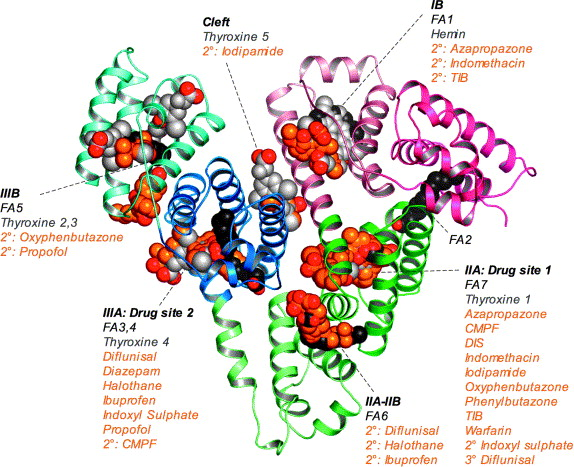
\includegraphics[width=0.49\textwidth]{figures/hsa_fig7_ghuman2005.jpg}
	\caption{\textbf{Summary of the ligand-binding capability of Human serum albumin structural studies to date.} Ligands are depicted in space-filling representation; oxygen atoms are coloured red; all other atoms in fatty acids (myristic acid), other endogenous ligands (hemin, thyroxin) and drugs are coloured dark-grey, light grey and orange, respectively. From figure 7 of \cite{Ghuman2005a}.}
	\label{figure:albumin}
	\todo[inline,color=red!40]{show small molecules we will use}
\end{figure} 
% \subsubsection*{Methods}

\subsubsubsection{Subaim 3.1: Extend semi-grand canonical ensemble alchemical free energy calculation tools}
At current time, a framework to perform semi-grand canonical ensemble simulations with multiple ligands does not exist. Therefore we will extend the framework of alchemical free energy calculations to include the potential for multiple (possibly weak) binding events using a semi-grand canonical ensemble formalism. 
The total number of ligands bound to a target is governed by its chemical potential, $\mu$. 
\todo[inline,color=red!40]{This isn't really the main idea here.  The key idea is that we need to compute the free energy of having 0, 1, 2, 3... ligands bound to the protein for some sort of standard state volume. Then, for a given ligand concentration, we can compute the probability that a given macromolecule will have 0, 1, 2, 3... ligands bound.  We can even go further and say something about cooperativities between sites, etc.)}

Alchemical methods will allow us to insert new copies of ligands into our simulation without driving the system far away from equilibrium. 

\todo[inline]{Using NCMC?, Does this take care of larger ligands?, Implicit v Explicit solvent}	

\subsubsubsection{Subaim 3.2: Validate computational predictions by applying Bayesian model selection on ITC  experiments of HSA and a series of NSAIDS}
To provide validation of our computational results, we will \textbf{perform ITC experiments on HSA}. Binding stoichiometry is not known a priori, yet if we want to deconvolute characteristics such as binding affinities for different sites, we need to model multiple binding sites with multiple affinities.
\todo[inline,color=red!40]{stoichiometry is too primitive to describe multiple binding sites with varying affinity}

\textbf{Using the predicted affinities and stoichiometry from alchemical free energy calculations, we can design ITC experiments} that can provide maximal information on the actual associations. 

To analyze the experiments, we will have to develop new methodology. 
Origin, a conventional ITC analysis software package uses cooperativity parameters $n_i$ to describe multiple binding sites\cite{MicroCal2004a} up to a maximum of two. SEDPHAT additionally uses terms describing ``incompetent fractions'' of experimental components \cite{Houtman2007a,Zhao2015b} and can deal with up to 3 sites.
We will \textbf{extend our Bayesian analysis tools} with the capacity to select between possible association models \textbf{without limiting the number of distringuishable sites or binding stoichiometry}. At the same time \textbf{it will be able to distinguish errors in the concentrations of the prepared solutions from changes in stoichiometry}, unlike the simple Origin models. 

\todo[inline,color=red!40]{correlated uncertainty estimates}

Individual binding associations can be modeled as
\todo[inline,color=red!40]{formulate a model that allows for multiple different associations, affinities etc}

\subsubsection*{Expected results}
Alchemical free energy calculations can suggest the number of predicted interaction sites, as well as provide estimates for the affinity of each individual site.
This allows us to study the predicted interactions at an atomistic scale, as well as design experiments at concentrations that will provide the most detailed information, for ITC experiments that can observe multiple drugs binding to HSA at the same time, or binding to multiple sites.

\todo[inline,color=red!40]{expected for overall aim?}

Our Bayesian ITC analysis methodology will then enable us to predict binding affinities to HSA with its multiple binding sites. We will be able to deconvolute the heat effects of multiple species, as well as multiple binding sites.

\subsubsection*{Pitfalls and alternatives}
Binding sites with multiple affinities might be hard to measure accurately with ITC if the affinities are very different. We can perform dynamic range experiments which search multiple ranges of concentration and detect binding sites. Then, using Bayesian experimental design, we can perform adaptive experiments that will yield new information that can describe all the features detected.

\todo[inline,color=red!40]{competition experiments could be helpful, push out weak binder with strong binder?}

\section*{Conclusion}
The aims of this proposal contribute to the limited set of tools available to deal with protein-ligand interactions in special, but not rare, cases where conventional tools provide no theoretical framework. Using Bayesian methodology will provide reliable uncertainty estimates on experimental data, which in turn will enable the distinction between theoretical model errors and experimental errors.

% refs
\printbibliography

\end{document}
